\tikzset{
    partial ellipse/.style args={#1:#2:#3}{
        insert path={+ (#1:#3) arc (#1:#2:#3)}
    }
}
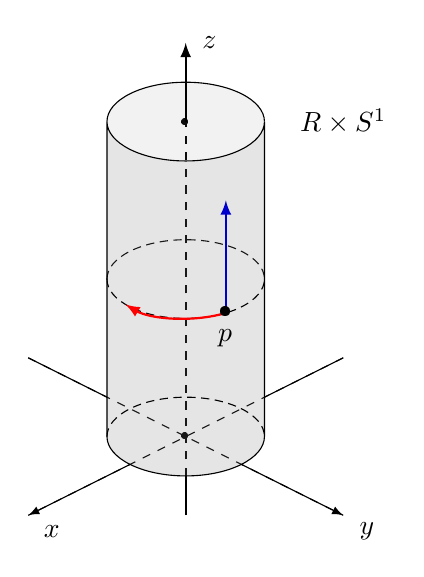
\begin{tikzpicture}
\draw[-latex] (2,1)-- (-2,-1)  ;
\draw[-latex]  (-2,1)--(2,-1)  ; 

 \draw[fill=white,draw=none] (-1,4) -- (-1,0) arc (180:360:1cm and 0.5cm) -- (1,4) arc (-180:0:-1cm and 0.5cm) ;
\draw[fill=white,draw=none] (0,4) ellipse (1cm and 0.5cm);
\draw[-,thick, dashed] (0,-0.5) -- (0,4) ;
\draw[dashed] (2,1)-- (-2,-1)  ;
\draw[dashed]  (-2,1)--(2,-1)  ;
\draw[-,thick] (0,-1) -- (0,-0.5) ;
\node at (0,0) {\tiny\textbullet};
\node at (0,4) {\tiny\textbullet};
  \draw[densely dashed] (-1,2) arc (180:0:1cm and 0.5cm);

  \draw[fill=gray,fill opacity = 0.1,draw=none] (0,4) ellipse (1cm and 0.5cm);
 
  \draw[fill=gray,fill opacity = 0.2] (-1,4) -- (-1,0) arc (180:360:1cm and 0.5cm) -- (1,4) arc (-180:0:-1cm and 0.5cm) ;
  \draw[densely dashed] (-1,0) arc (180:0:1cm and 0.5cm);
  \draw(-1,4) arc (180:0:1cm and 0.5cm);

  \draw[densely dashed]  (-1,2) arc (-180:0:1cm and 0.5cm);
  \draw[thick, red, -latex] (0,2) [partial ellipse=-60:-140:1cm and 0.5cm];
 \draw[thick, blue!80!black,-latex] (0.51,1.57)-- (0.51,3);
  \node at (2,4) {$\mathbb{R}\times\mathbb{S}^1$};
  \node at (2+0.3,-1-0.2) {$y$};
  \node at (-2+0.3,-1-0.2) {$x$};
  \node at (0.3,5) {$z$};
   \node at (0.5,1.25) {$p$};
  \draw[-latex,thick] (0,4) -- (0,5) ;
  \node at (0.51,1.57){\textbullet};
;\end{tikzpicture}
